

%----------------------------------------------------------------------------------------
%	PACKAGES AND OTHER DOCUMENT CONFIGURATIONS
%----------------------------------------------------------------------------------------

\documentclass[12pt]{article}

\usepackage{polski}
\usepackage[polish]{babel}
\usepackage[utf8]{inputenc}
\usepackage{datetime}  
\usepackage{graphicx}
\usepackage{tikz}
\usepackage{amsmath}
\usepackage{epstopdf}
\usepackage{multirow}
\usepackage{tabularx}
%\usepackage[colorlinks=true]{hyperref}
%\usepackage[all]{hypcap}
%\usepackage{showframe} 
\usepackage{geometry}
 \geometry{
 a4paper, 
 left=20mm,
 right=20mm,
 top=20mm,
 bottom=20mm,
 }
 
%----------------------------------------------------------------------------------------
 
%----------------------------------------------------------------------------------------
% DATES
%----------------------------------------------------------------------------------------

\renewcommand{\dateseparator}{.}
\newdate{exercise_date}{30}{04}{2014}

%----------------------------------------------------------------------------------------

%----------------------------------------------------------------------------------------
% TIKZ PACKAGES
%----------------------------------------------------------------------------------------

\usetikzlibrary{arrows}

%----------------------------------------------------------------------------------------

\begin{document}
 
\begin{titlepage}

\newcommand{\HRule}{\rule{\linewidth}{0.5mm}}
% Defines a new command for the horizontal lines, change thickness here

\center
% Center everything on the page
 
%----------------------------------------------------------------------------------------
%	LOGO SECTION
%----------------------------------------------------------------------------------------


\includegraphics[width=6cm]{../res/img/logo.png}\\[1cm]
% Include a department/university logo - this will require the graphicx package
 
%----------------------------------------------------------------------------------------
 
%----------------------------------------------------------------------------------------
%	HEADING SECTIONS
%----------------------------------------------------------------------------------------

\textsc{\LARGE Akademia Górniczo-Hutnicza \\[0.2cm]
im. Stanisława Staszica w Krakowie}\\[1.5cm]
% Name of your university/college

\textsc{\Large Podstawy Automatyki}\\[0.5cm]
% Major heading such as course name

%----------------------------------------------------------------------------------------
%	TITLE SECTION
%----------------------------------------------------------------------------------------

\HRule \\[0.5cm]
{ \huge \bfseries Dyskretne układy regulacji \\[0.3cm] oraz \\[0.5cm] Analiza
serwomechanizmu \\[0.2cm] przekaźnikowego z wykorzystaniem płaszczyzny
fazowej}\\[0.3cm]
% Title of your document
\HRule \\[1.5cm]
 
%----------------------------------------------------------------------------------------
%	AUTHOR SECTION
%----------------------------------------------------------------------------------------

% \begin{minipage}{0.4\textwidth}
% \begin{flushleft} \large
% \emph{Author:}\\
% Konrad \textsc{Adasiewcz} % Your name
% \end{flushleft}
% \end{minipage}
% ~
% \begin{minipage}{0.4\textwidth}
% \begin{flushright} \large
% \emph{Supervisor:} \\
% dr inż. Paweł \textsc{Rotter} % Supervisor's Name
% \end{flushright}
% \end{minipage}\\[4cm]

% If you don't want a supervisor, uncomment the two lines below and remove the section above
\flushright
\Large \emph{Autorzy:}\\
Konrad \textsc{Adasiewcz}\\[0.1cm] % Your name
Michał \textsc{Maciejewski}\\[3cm] % Your name

%----------------------------------------------------------------------------------------
%	DATE SECTION
%----------------------------------------------------------------------------------------
Data wykonania ćwiczenia: \\
{\large \displaydate{exercise_date}}\\[1cm]


\vfill % Fill the rest of the page with whitespace

\end{titlepage} 

\section{Wstęp}

\subsection{Cel ćwiczenia} 

Celem ćwiczenia jest zapoznanie się z badaniem stabilności zamkniętego układu regulacji automatycznej z 
wykorzystaniem kryterium Nyquista oraz kryterium Hurwitza. Podczas wykonywania
ćwiczenia badamy zamknięty układ regulacji składający się z obiektu o
transmitancji:

\begin{equation}
	G_o(s)=\frac{10}{s^3+2s^2+2s+1}
\end{equation}

oraz ciągłego regulatora \textsc{PID} o transmitancji:

\begin{equation}
	G_r(s)=k\left(1+\frac{1}{T_is}+\frac{T_ds}{Ts+1}\right)
\end{equation}

Przyjmujemy wyjściowe parametry regulatora $k=2[-]$, $T_i=1[s]$, $T_d=0.5[s]$,
$T=0.01[s]$(parametr stały regulatora).

\begin{figure}[!htb]
	\begin{center}
		\begin{tikzpicture}[scale=1.5]
	\draw[-latex, ultra thick]
		(0,0)	--	node[scale=1.2,above]{$Z(s)$}
		(1.5,0)	node[above left]{+};
	\draw
		(1.75,0)	circle (0.25)
		+(45:0.25)	--
		+(-135:0.25)
		+(-45:0.25)	--
		+(135:0.25);
	\draw[-latex, ultra thick]
		(1.75,-2)	--
		(1.75,-0.25)	node[below left]{-};
	\draw[-latex, ultra thick]
		(2,0)	--	node[scale=1.2,above]{$E(s)$}
		+(1,0);
	\draw[rounded corners]
		(3,-1)	rectangle
		+(2,2)
		+(1,1)	node[scale=2]{$G_r(s)$};
	\draw[-latex, ultra thick]
		(5,0)	--	node[scale=1.2,above]{$U(s)$}
		+(1,0);
	\draw[rounded corners]
		(6,-1)	rectangle
		+(2,2)
		+(1,1)	node[scale=2]{$G_o(s)$};
	\draw[-latex, ultra thick]
		(8,0)	--	node[scale=1.2,above]{$Y(s)$}
		+(2,0);
	\draw[ultra thick]
		(9,0)		--
		++(0,-2)	--
		++(-7.25,0);
	\filldraw[color=black]
		(9,0) circle (0.1);
	
\end{tikzpicture}
	\end{center}
	\caption{Schemat badanego układu}
\end{figure}

Należy tak manipulować pojedynczymi parametrami regulatora aby zamknięty układ
regulacji był opisany stabilną transmitancją operatorową.

\subsection{Stabilność}

Stabilność układu dynamicznego determinuje rozkład biegunów jego transmitancji.
Tj. jeśli wszystkie bieguny transmitancji mają niedodatnie części rzeczywiste
oraz co najwyżej jeden biegun jest zerowy, to układ nazywamy stabilnym.
Dodatkowo jeśli wszystkie bieguny mają części rzeczywiste \textit{ujemne}, to
układ nazywamy stabilnym asymptotycznie. Jeśli przynajmniej jeden biegun transmitancji ma część
rzeczywistą dodatnią, to układ nazywamy niestabilnym.

Do rozstrzygania położenia pierwiastków na płaszczyźnie zespolonej $s$, służą
kryteria stabilności, w szczególności badane kryteria Hurwitza oraz pośrednio
informację o rozkładzie biegunów transmitancji układu zamkniętego daje nam
częstotliwościowe kryterium Nyquista.

\newpage

\section{Kryterium Hurwitza}

Kryterium Hurwitza pozwala na stwierdzenie czy wszystkie pierwiastki wielomianu
leżą w lewej półpłaszczyźnie zespolonej $s$. Tak jest wtedy i tylko wtedy gdy
dla wielomianu:

\begin{equation*}
	a_ns^n+a_{n-1}s^{n-1}+\ldots+a_1s+a_0=0
\end{equation*}

Są spełnione następujące warunki:

\begin{itemize}
  \item Dla każdego $i=0\ldots n$, $a_i\neq 0$, oraz $a_i$ są tego samego znaku
  \item Dla każdego $i=1\ldots n$, $H_i>0$
\end{itemize}

Gdzie $H_i$ są wiodącymi minorami głównymi macierzy Hurwitza wielomianu,
zdefiniowanej następująco:

\begin{equation}
	H^{n\times n}=
	\begin{bmatrix}
		a_{n-1} & a_{n-3} & a_{n-5} & \ldots  & 0 \\
		a_{n}   & a_{n-2} & a_{n-4} & \ldots  & 0 \\
		0       & a_{n-1} & a_{n-3} &         & \vdots \\
		\vdots  & \vdots  &         & \ddots  & 0 \\
		0       & 0       & \ldots  & a_{2} & a_0 \\
	\end{bmatrix}
	\label{mat:hurwitz}
\end{equation}

Dodatkowo jeśli istnieje wiodący minor główny $H_j=0$ to istnieje pierwiastek
wielomianu czysto urojony.

Kryterium Hurwitza rozstrzyga więc o stabilności asymptotycznej układu
dynamicznego, na podstawie jego transmitancji operatorowej. A jeśli istnieje
wiodący minor główny zerowy to układ znajduje się na granicy stabilności.

\newpage

\section{Kryterium Nyquista}

Kryterium Nyquista rozstrzyga czy zamknięty układ regulacji jest stabilny na
podstawie charakterystyki częstotliwościowej układu otwartego. Mówi ono iż:

\begin{itemize}
  \item Jeżeli układ otwarty jest stabilny:
\end{itemize}

Układ zamknięty będzie stabilny wtedy i tylko wtedy, gdy charakterystyka
amplitudowo-fazowa układu otwartego nie obejmuje punktu $(-1,j0)$ na
płaszczyźnie zespolonej. Ściślej - przechodząc po charakterystyce
częstotliwościowej w kierunku rosnącej częstotliwości musimy punkt
$(-1,j0)$ mieć po lewej stronie. Gdy charakterystyka ta przechodzi przez punkt
$(-1;j0)$, to układ jest na granicy stabilności.

\begin{itemize}
  \item Jeżeli układ otwarty jest niestabilny i ma $k$ pierwiastków w prawej
półpłaszczyźnie zespolonej:
\end{itemize}

Układ zamknięty będzie stabilny wtedy i tylko wtedy, gdy charakterystyka
amplitudowo-fazowa układu otwartego obejmuje $\frac{k}{2}$ razy punkt $(-1, j0)$
na płaszczyźnie zespolonej. Inaczej: Promień wodzący wychodzący od punktu
$(-1,j0)$ i skierowany w stronę charakterystyki zakreśla kąt $\frac{k}{2}\pi$
przy $\omega$ zmieniającej się od $0$ do $\infty$. Kierunkiem dodatnim jest kierunek
przeciwny do ruchu wskazówek zegara.

\vspace{1cm}

Kryterium Nyquista jest chętnie wykorzystywane do badania stabilności układu
zamkniętego przy braku znajomości jego transmitancji, ponieważ można
rozstrzygnąć o stabilności układu zamkniętego, posiadając jedynie
charakterystykę częstotliwościową układu otwartego, którą można wyznaczyć
doświadczalnie. Układ otwarty musi być jednak stabilny aby móc wygodnie
skorzystać z kryterium Nyquista.

My znamy transmitancję obiektu oraz regulatora, znamy więc również transmitancję
układu otwartego, zbadamy więc jego stabilność korzystając z kryterium Hurwitza.

Transmitancja układu otwartego dla przyjętych nastaw regulatora ma postać:

\begin{equation}
	G_{ot}(s)=\frac{10.2s^2+20.2s+20}{s(0.01s^4+1.02s^3+2.02s^2+2.01s+1)}
\end{equation}

Widać, że jednym z pierwiastków mianownika jest $s=0$, więc układ otwarty jest
układem astatycznym(o charakterze całkującym). Pozostały czynnik wielomianowy
mianownika spełnia warunek konieczny kryterium Hurwitza, oraz jego macierz
Hurwitza posiada wszystkie wiodące minory główne dodatnie, to też wszystkie jego
pierwiastki posiadają ujemne części rzeczywiste. Układ otwarty jest więc
stabilny, nie jest jednak stabilny asymptotycznie. Do badania
stabilności układu zamkniętego korzystamy więc z pierwszego kryterium Nyquista.








\newpage

\section{Odpowiedzi skokowe i kryteria stabilności}

\subsection{Układ wyjściowy}

\subsubsection{Kryterium Hurwitza}

Transmitancja układu zamkniętego z wyjściowymi parametrami regulatora ma postać:

\begin{equation}
	G_{z}(s)=\frac{10.2s^2+20.2s+20}{0.01s^5+1.02s^4+2.02s^3+12.21s^2+21.2s+20}
\end{equation}

Mianownik spełnia warunek konieczny Hurwitza, można więc ułożyć macierz
\eqref{mat:hurwitz} i sprawdzić czy wszystkie jego wiodące minory główne są
dodatnie. Dla takich współczynników macierz Hurwitza ma postać:

\begin{equation}
	H=
	\begin{bmatrix}
		 	1.02  	& 	12.21 	&  	20 		&      0        	& 0	\\
    		0.01  	&  	2.02  	& 	21.2	&      0        	& 0	\\
    	    0    	&	1.02  	& 	12.21  	& 		20  		& 0	\\
         	0    	&	0.01  	&  	2.02   	&		21.2  		& 0	\\
         	0       &  	0    	&	1.02   	&		12.21  		& 20
	\end{bmatrix}
\end{equation}

Wiodące minory główne tej macierzy to: $\{1.02;1.94;1.81;-35.56;-711.25\}$, więc
układ przy takiej konfiguracji parametrów regulatora jest niestabilny.

\newpage

\subsubsection{Kryterium Nyquista}

Jak widać na poniższej charakterystyce, przechodząc od częstotliwości niskich do
wysokich mijamy punkt $(-1, j0)$ z prawej strony, układ zamknięty będzie więc
niestabilny.

\begin{figure}[!htb]
	\begin{center}
		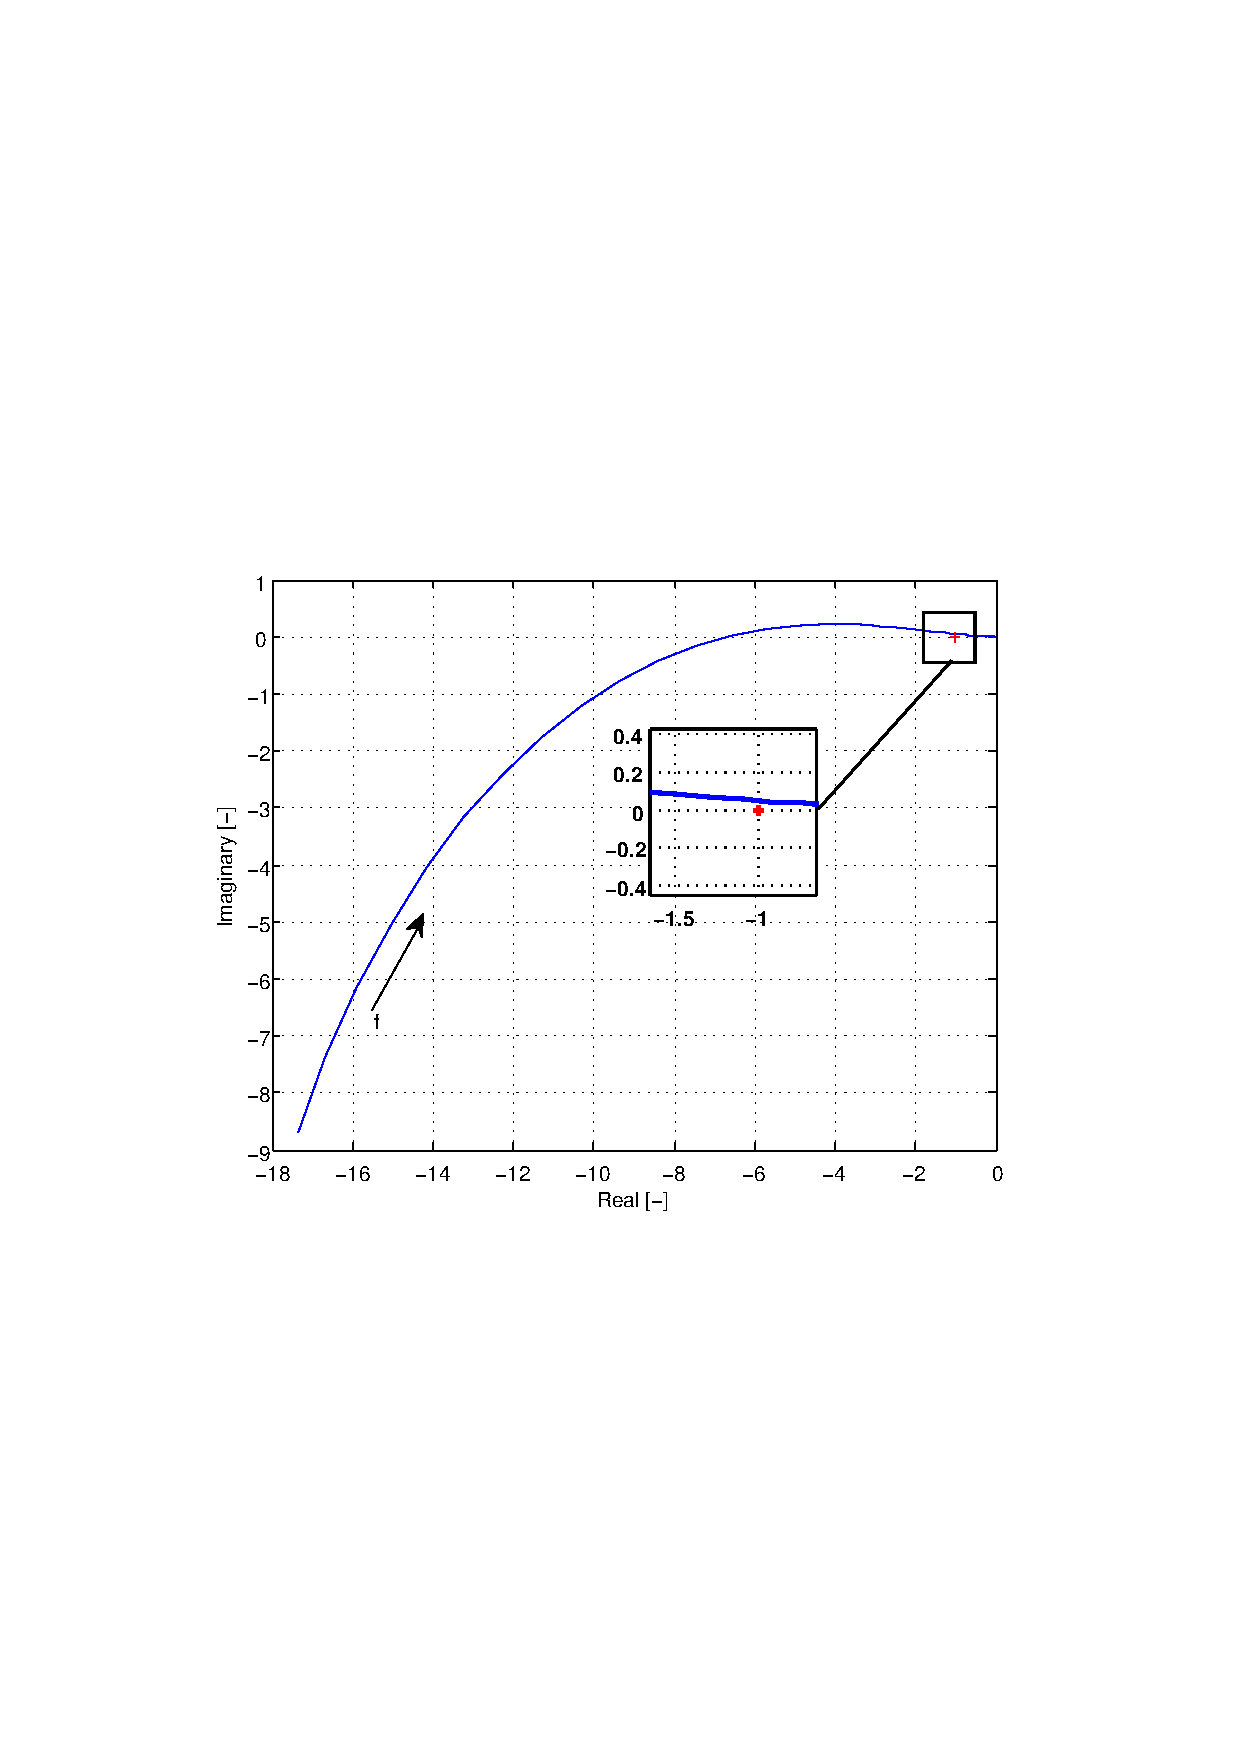
\includegraphics[trim=5cm 9cm 5cm 9cm]{../res/img/2-1-0,5_nyq.pdf} 
	\end{center}
	\caption{Charakterystyka Nyquista układu otwartego dla wyjściowych parametrów
	regulatora}
\end{figure}

\newpage

\subsubsection{Odpowiedź skokowa}

Kryteria stanowią, iż dla wyjściowych parametrów regulatora badany układ
zamkniętej regulacji będzie niestabilny, co powinno być widoczne na jego
odpowiedzi skokowej.

\begin{figure}[!htb]
	\begin{center}
		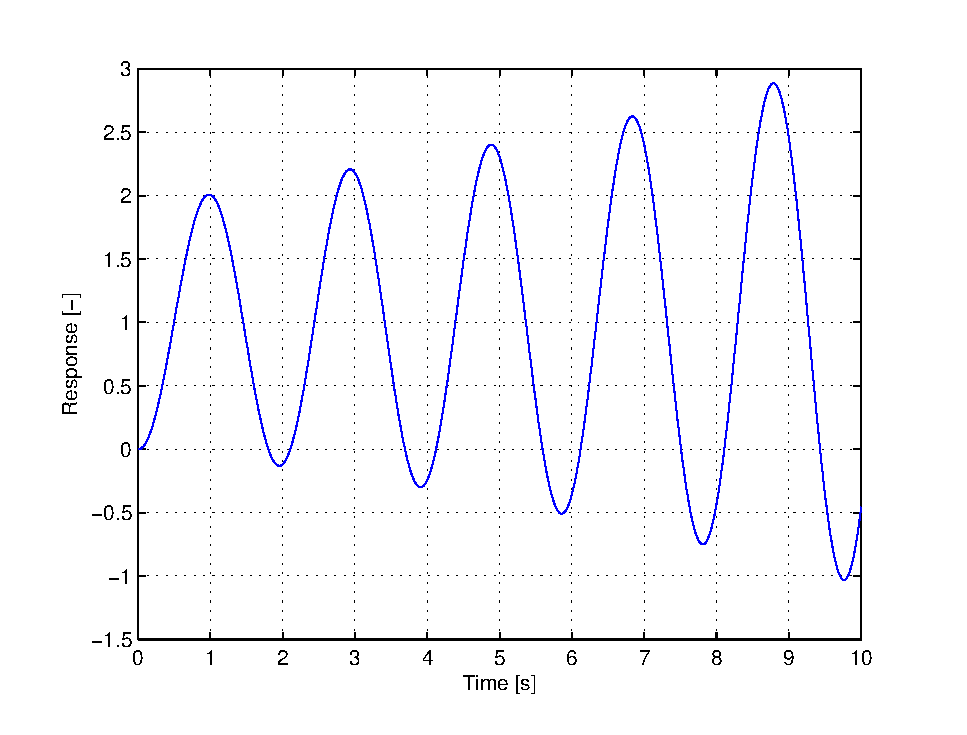
\includegraphics[width=15cm]{../res/img/2-1-0,5_resp.eps} 
	\end{center}
	\caption{Odpowiedź skokowa układu zamkniętego dla wyjściowych parametrów
	regulatora}
\end{figure}

Jak widać odpowiedź skokowa układu rozbiega się, co stanowi o poprawności
analizy stabilności układu kryteriami Hurwitza i Nyquista.








\newpage

\subsection{Parametr k}

Zmniejszając parametr $k$ regulatora można doprowadzić do ustabilizowania
układu. Metodą prób znaleźliśmy parametr $k$, dla którego układ znajduje się na
granicy stabilności $k_g=0.3[-]$, oraz idąc dalej - jest stabilny $k_s=0.1[-]$.
Poniżej zamieszczamy analizę kryteriów stabilnościowych dla tak dobranych
parametrów $k$.

\subsubsection{Kryterium Hurwitza}

Pominiemy postać transmitancji operatorowej, oraz zapis macierzy Hurwitza dla
zmienionych parametrów.

Wartości minorów dla $k=k_g$ to: $\{1.02;2.03;3.01;-0.03;-0.1\}$, więc kryterium
stwierdza, iż układ jest niestabilny. Lecz z uwagi na to, iż wartości ujemnych
minorów są bardzo małe można podejrzewać, iż układ będzie znajdował się w
okolicy granicy stabilności.

Wartości minorów dla $k=k_s$ to: $\{1.02;2.04;3.05;2.04;2.04\}$,
więc kryterium stwierdza, iż układ jest stabilny asymptotycznie.

\subsubsection{Kryterium Nyquista}

Jak widać poniższa charakterystyka, przechodzi przez punkt $(-1, j0)$ więc można
się spodziewać, iż układ będzie znajdować się na granicy stabilności.

\begin{figure}[!htb]
	\begin{center}
		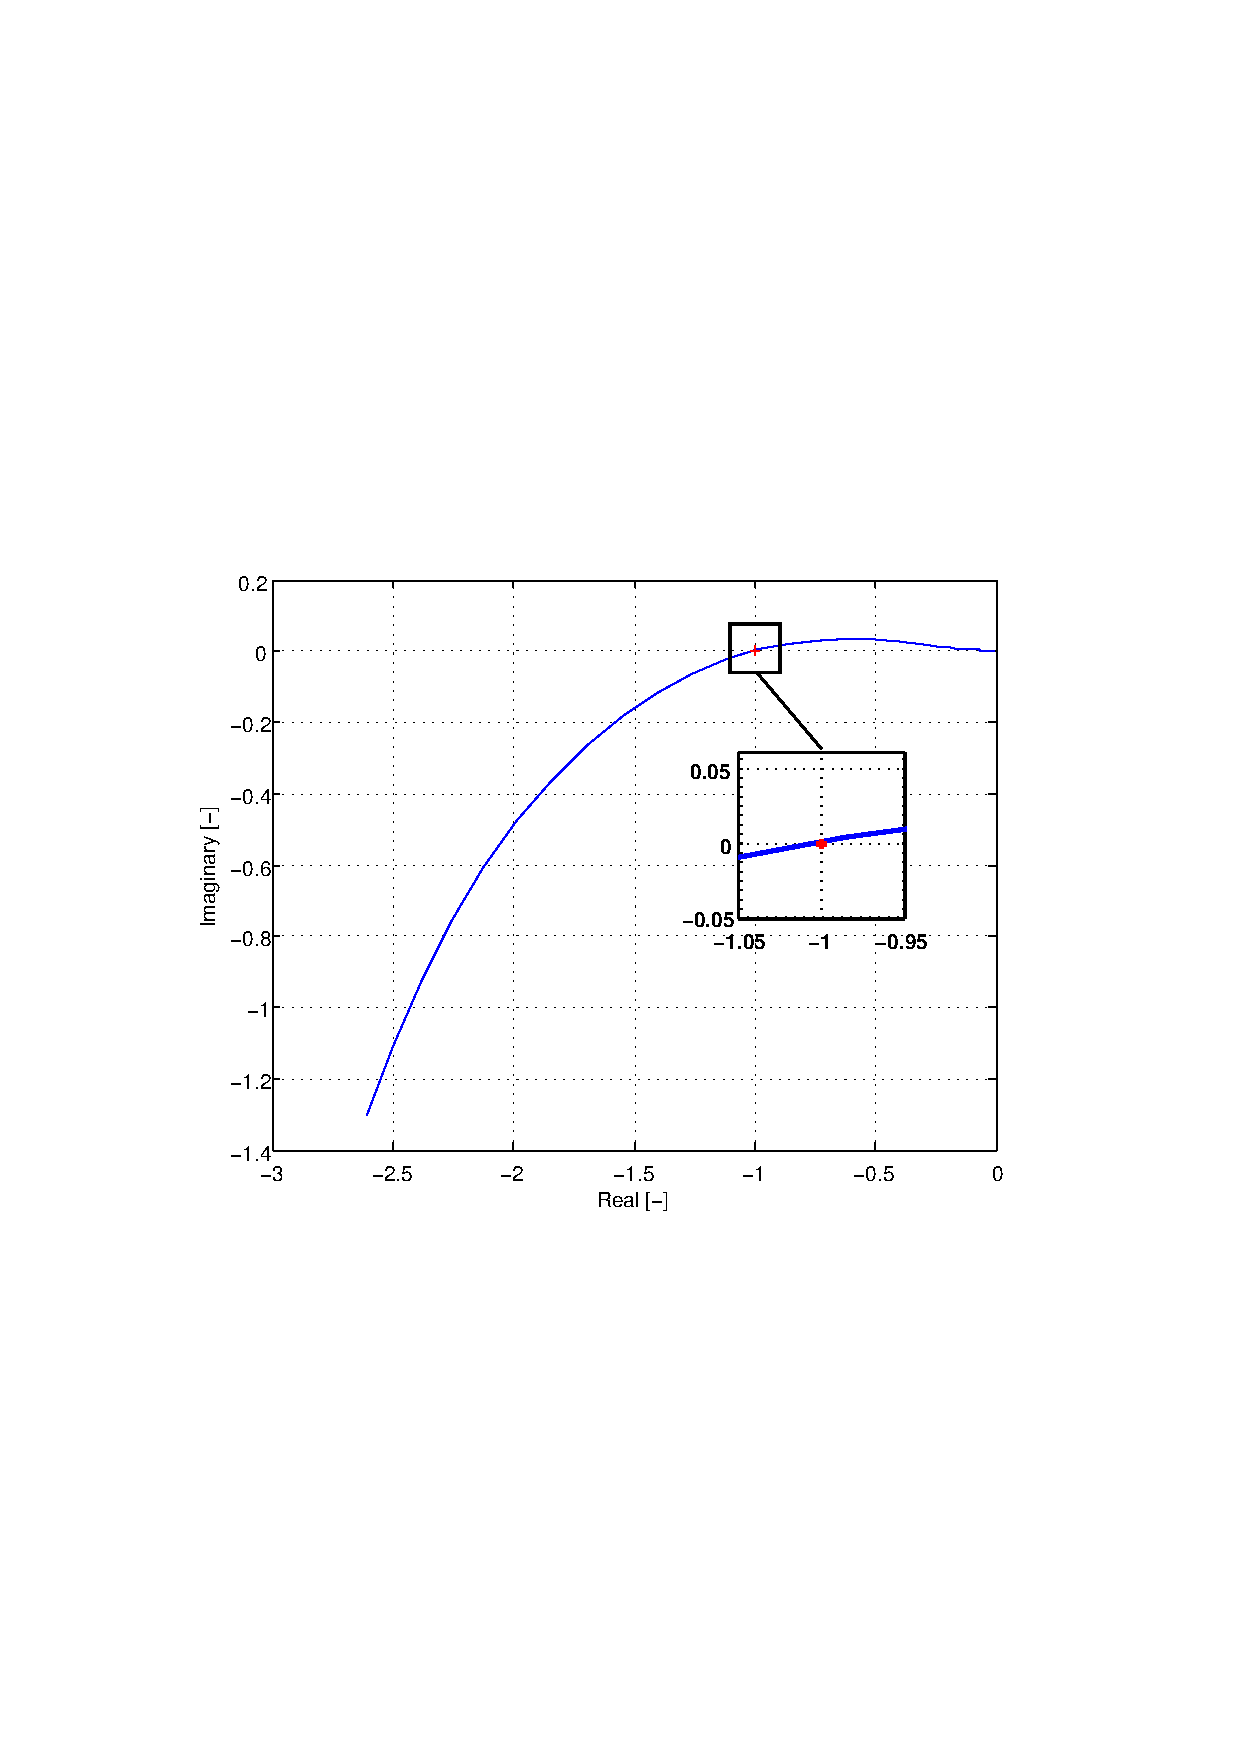
\includegraphics[trim=5cm 9cm 5cm 9cm]{../res/img/0,3-1-0,5_nyq.pdf} 
	\end{center}
	\caption{Charakterystyka Nyquista układu otwartego dla $k=k_g$}
\end{figure}

\newpage

W przypadku $k=k_s$ mijamy punkt $(-1, j0)$ mając go po lewej stronie, więc
kryterium stanowi, iż zamknięty układ regulacji będzie układem stabilnym.

\begin{figure}[!htb]
	\begin{center}
		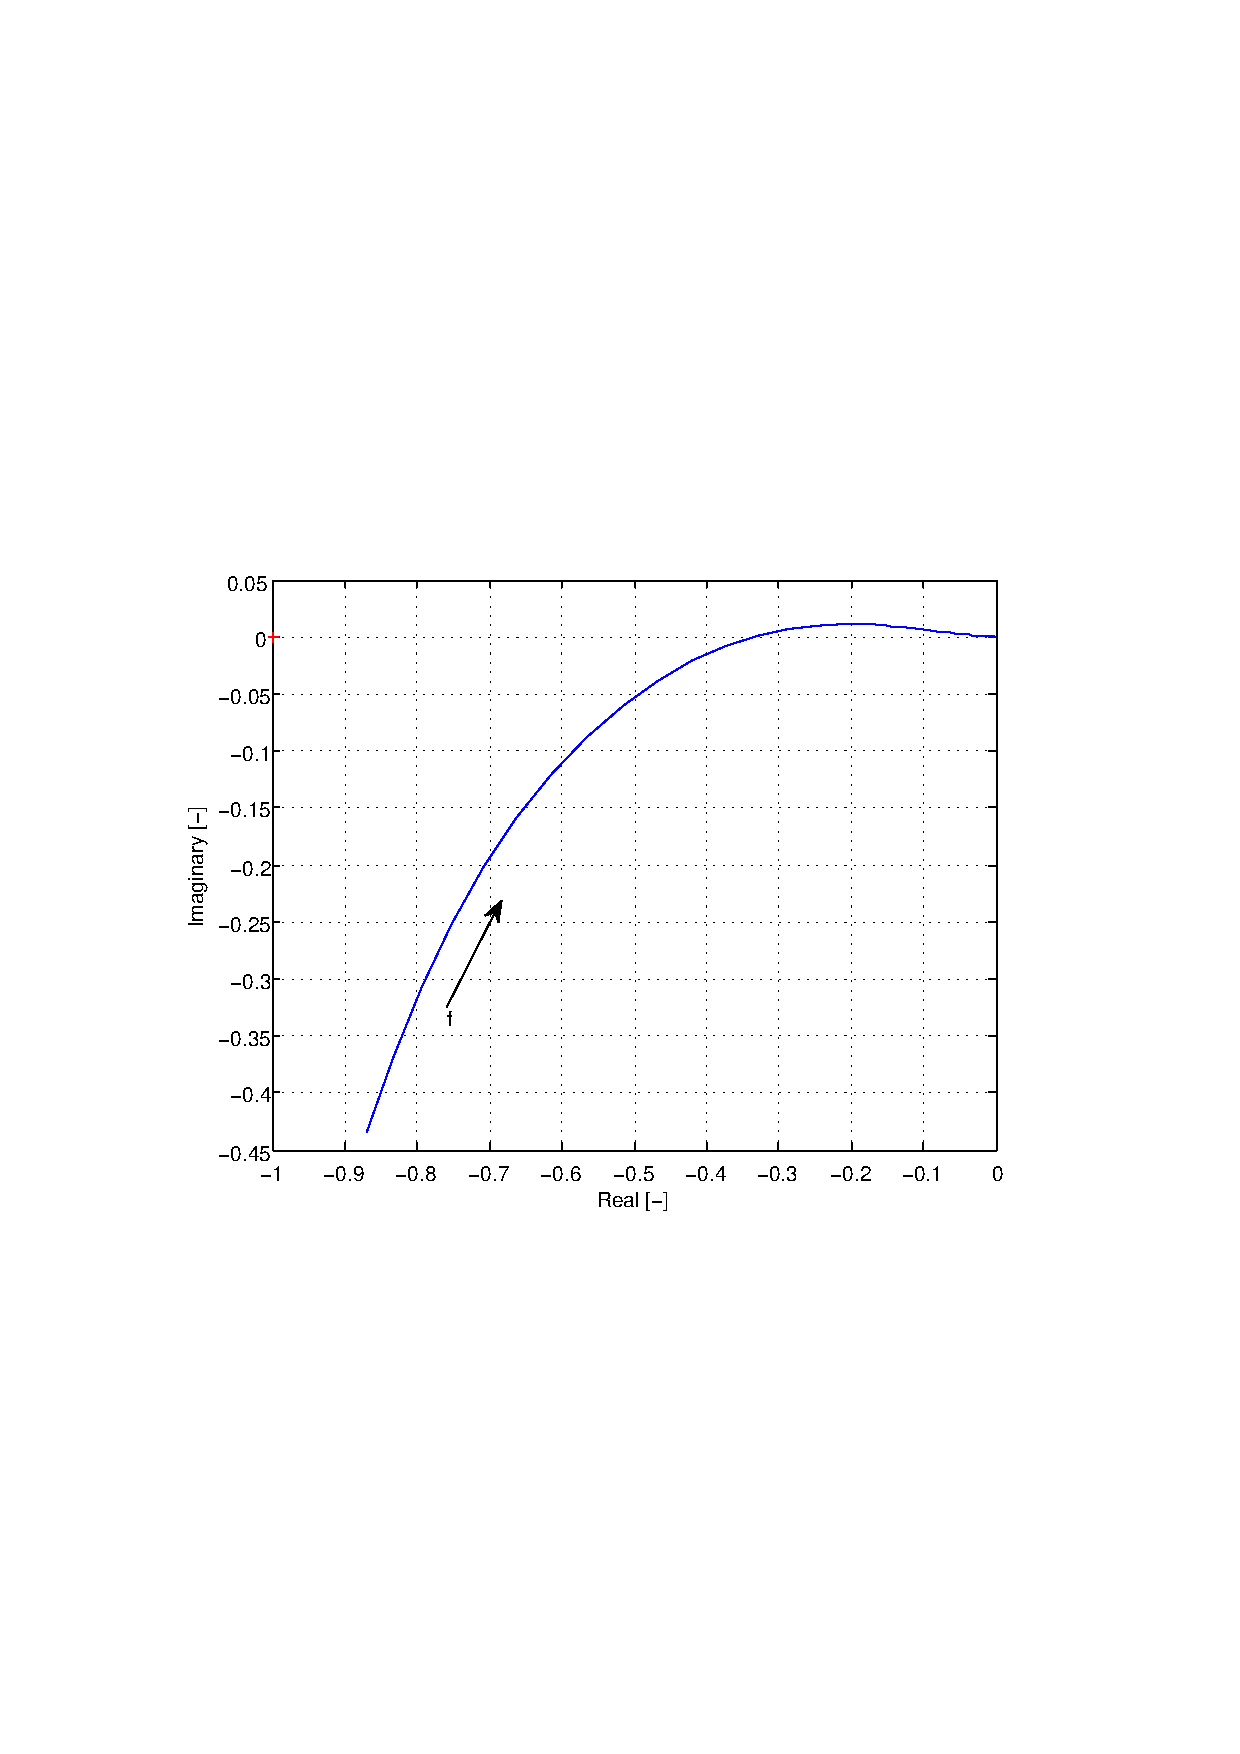
\includegraphics[trim=5cm 9cm 5cm 9cm]{../res/img/0,1-1-0,5_nyq.pdf} 
	\end{center}
	\caption{Charakterystyka Nyquista układu otwartego dla $k=k_s$}
\end{figure}

\newpage

\subsubsection{Odpowiedzi skokowe}

Poniżej zamieszczone są odpowiedzi skokowe dla nastaw $k$ regulatora dla których
kryteria stabilności stanowią, iż układ będzie na granicy stabilności, oraz
będzie stabilny.

\begin{figure}[!htb]
	\begin{center}
		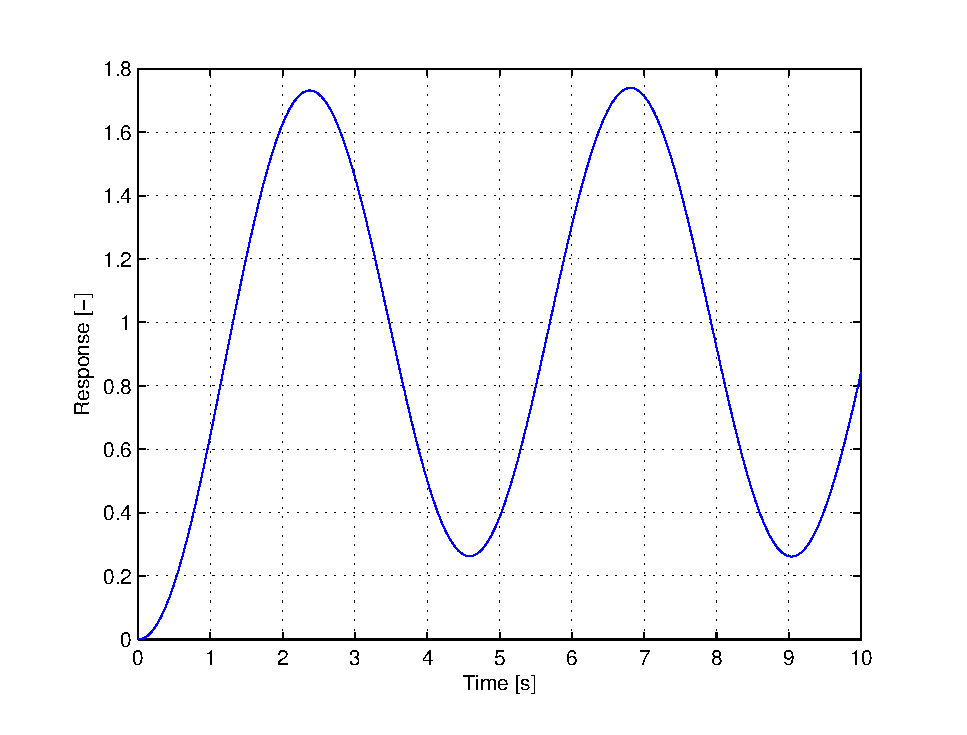
\includegraphics[width=12cm]{../res/img/0,3-1-0,5_resp.eps} 
	\end{center}
	\caption{Odpowiedź skokowa układu zamkniętego dla $k=k_g$}
\end{figure}

\begin{figure}[!htb]
	\begin{center}
		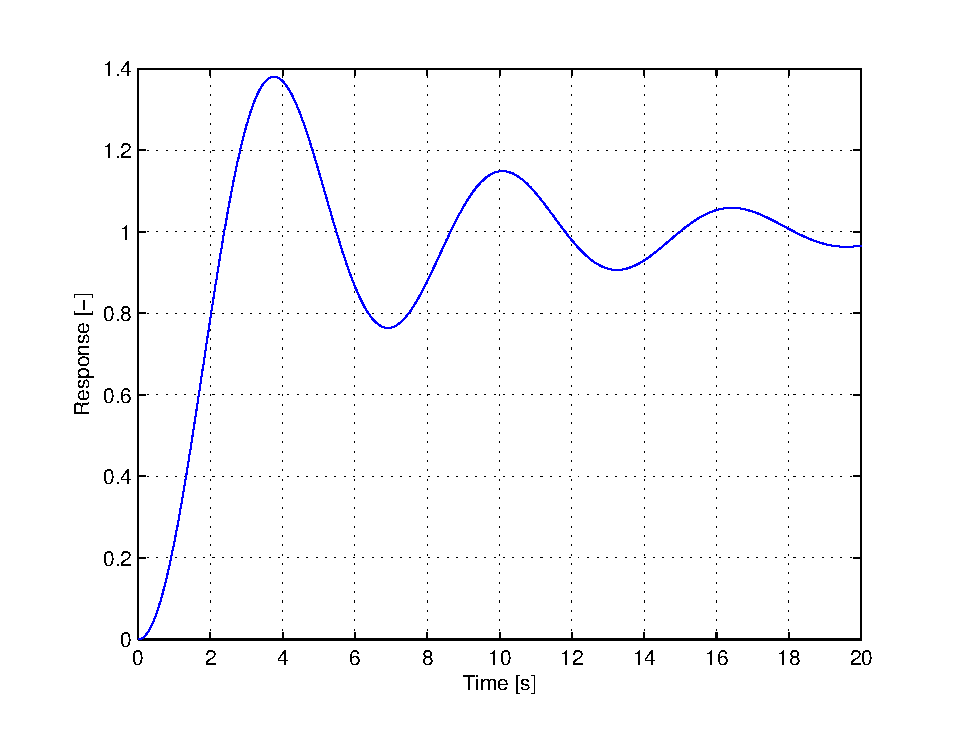
\includegraphics[width=12cm]{../res/img/0,1-1-0,5_resp.eps} 
	\end{center}
	\caption{Odpowiedź skokowa układu zamkniętego dla $k=k_s$}
\end{figure}







\newpage

\subsection{Parametr $T_i$}

Jak poprzednio, tym razem zwiększając parametr $T_i$ regulatora
można doprowadzić do ustabilizowania układu. Metodą prób znaleźliśmy parametr
$T_i$, dla którego układ znajduje się na granicy stabilności $T_{ig}=2[s]$, oraz
idąc dalej - jest stabilny $T_{is}=10[s]$. Poniżej zamieszczamy analizę
kryteriów stabilnościowych dla tak dobranych parametrów $T_i$.

\subsubsection{Kryterium Hurwitza}

Pominiemy postać transmitancji operatorowej, oraz zapis macierzy Hurwitza dla
zmienionych parametrów.

Wartości minorów dla $T_{i}=T_{ig}$ to: $\{2.04;7.75;14.52;20.96;419.33\}$,
więc kryterium stwierdza, iż układ jest stabilny. Jak się później okaże, układ
przy takim zestawie parametrów ciężko jest nazwać stabilnym(jest stabilny
jednak bardzo blisko granicy stabilności), co widać wyraźnie na charakterystyce
Nyquista.

Wartości minorów dla $T_{i}=T_{is}$ to: $\{10.2;193;1817;308085;6161713\}$,
więc kryterium stwierdza, iż układ jest stabilny asymptotycznie.

\subsubsection{Kryterium Nyquista}

Jak widać dla $T_{i}=T_{ig}$ poniższa charakterystyka, przechodzi przez punkt
$(-1, j0)$ więc układ będzie znajdować się na granicy stabilności.

\begin{figure}[!htb]
	\begin{center}
		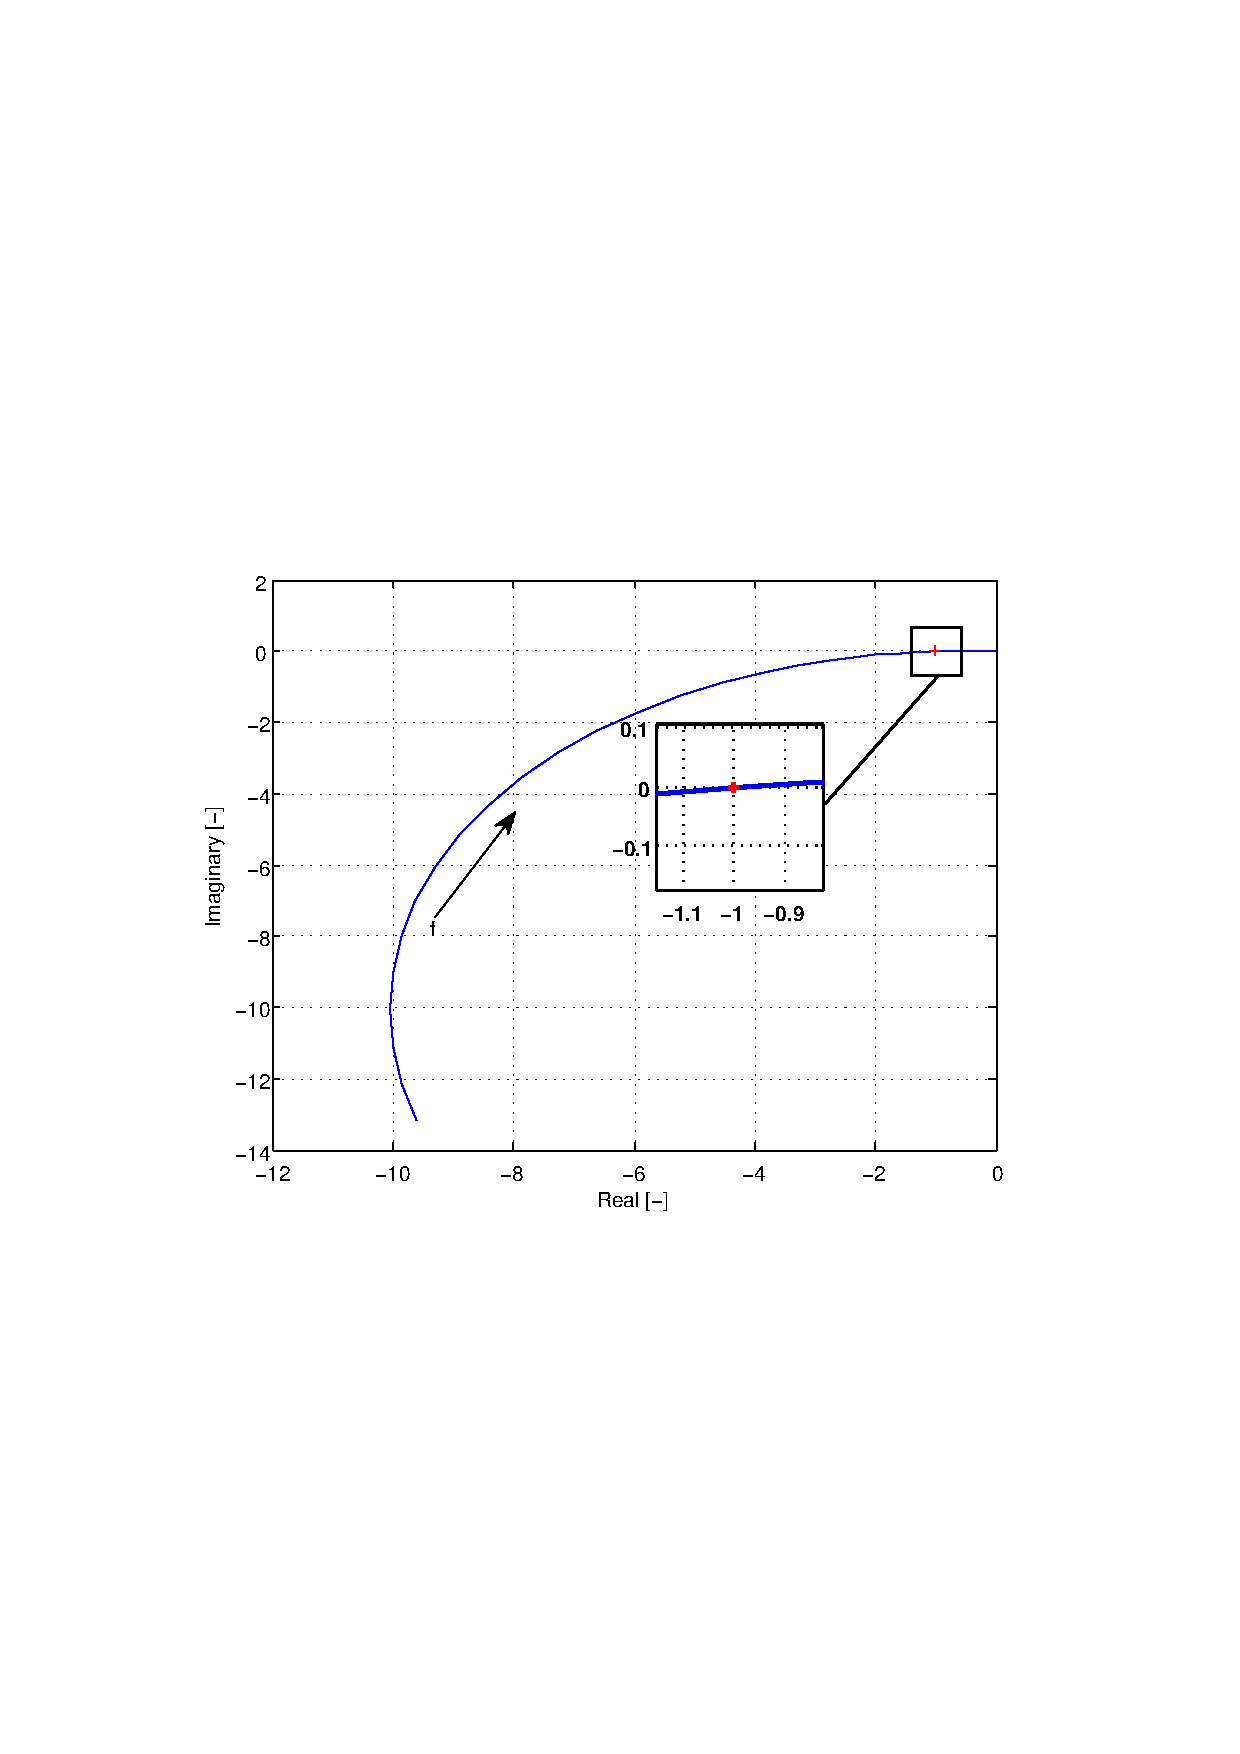
\includegraphics[trim=5cm 9cm 5cm 9cm]{../res/img/2-2-0,5_nyq.pdf} 
	\end{center}
	\caption{Charakterystyka Nyquista układu otwartego dla $T_{i}=T_{ig}$}
\end{figure}

\newpage

W przypadku $T_{i}=T_{is}$ mijamy punkt $(-1, j0)$ mając go po lewej stronie, więc
kryterium stanowi, iż zamknięty układ regulacji będzie układem stabilnym. Warto
zauważyć, iż pomimo że mijamy punkt $(-1, j0)$ ze strony zapewniającej
stabilność, przechodzimy bardzo blisko niego, co pozwala podejrzewać, iż mimo że
układ będzie stabilny to jednak jego charakter będzie nosił znamiona
niestabilności.

\begin{figure}[!htb]
	\begin{center}
		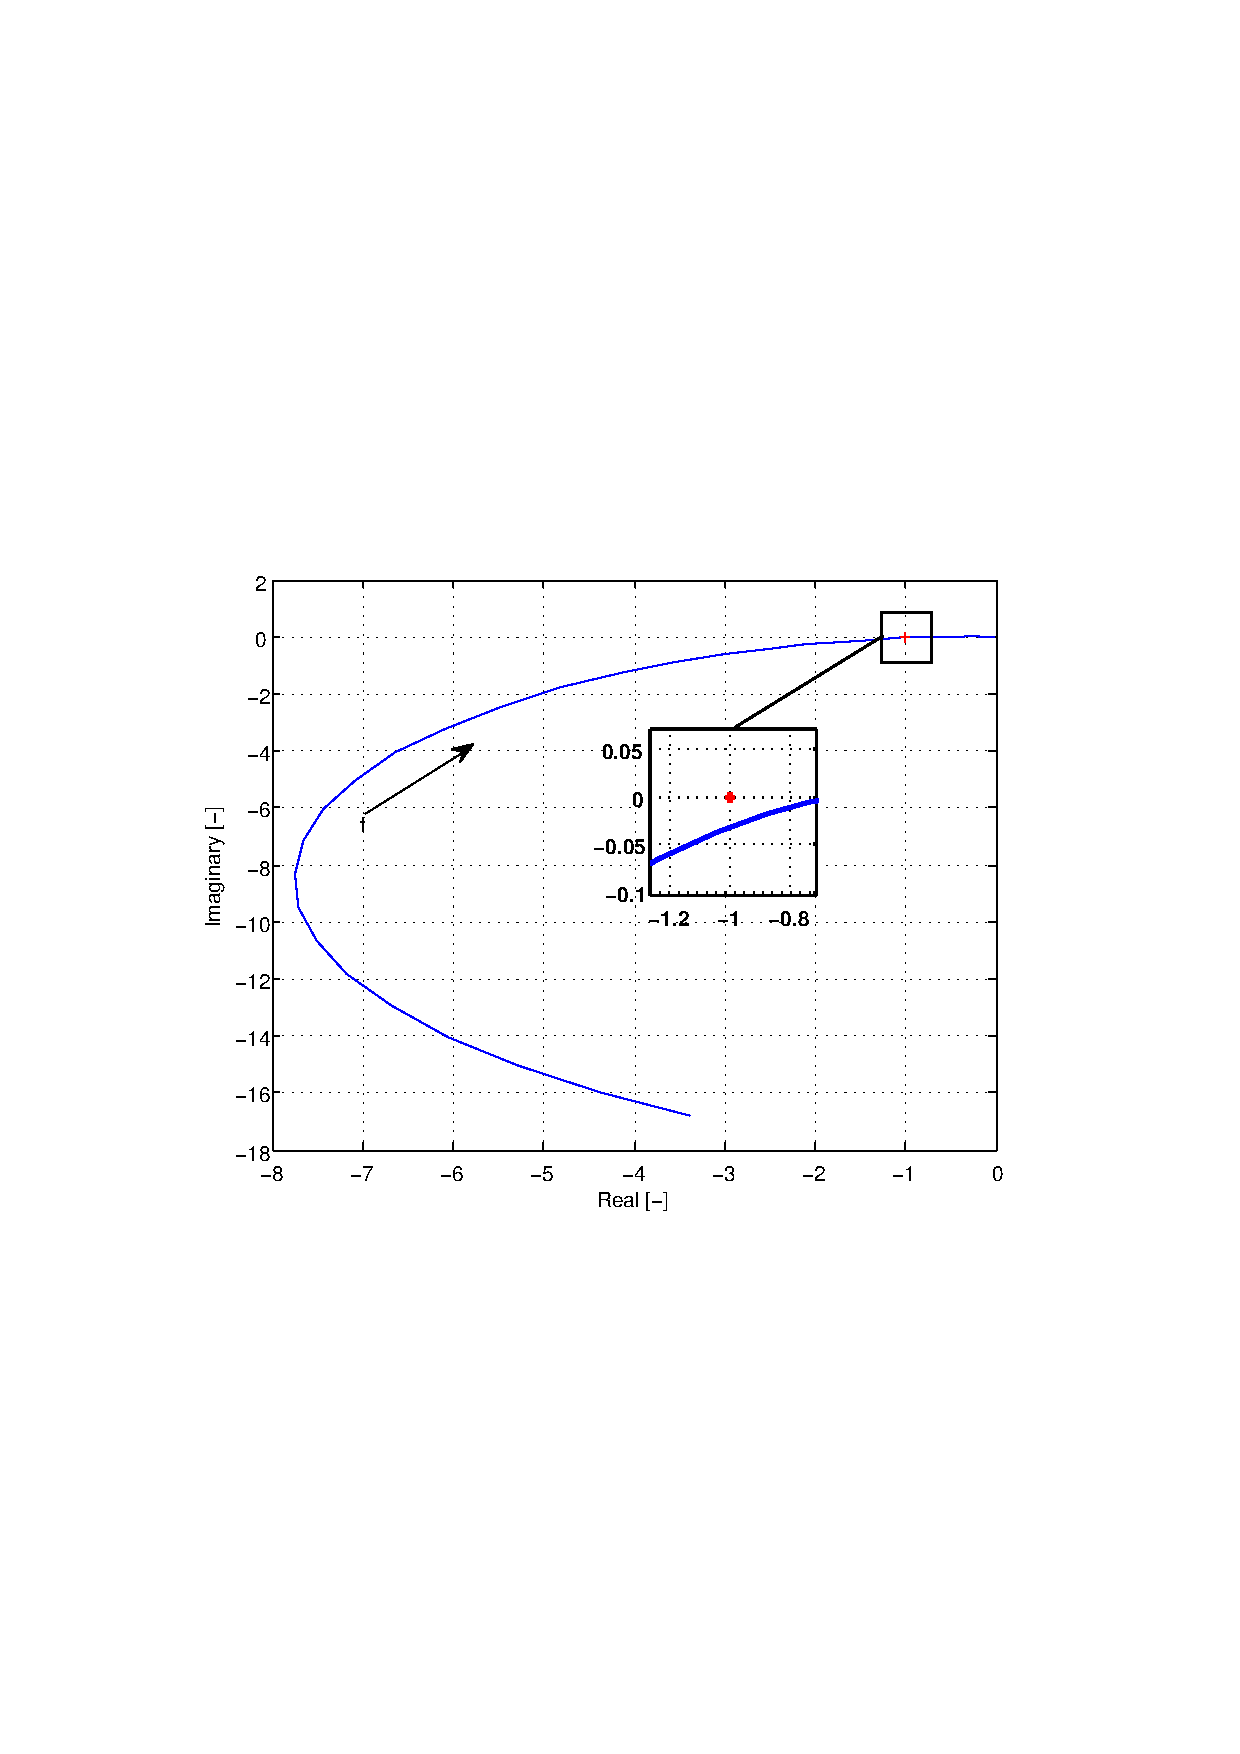
\includegraphics[trim=5cm 9cm 5cm 9cm]{../res/img/2-10-0,5_nyq.pdf} 
	\end{center}
	\caption{Charakterystyka Nyquista układu otwartego dla $T_{i}=T_{is}$}
\end{figure}

\newpage

\subsubsection{Odpowiedzi skokowe}

Poniżej zamieszczone są odpowiedzi skokowe dla nastaw $T_i$ regulatora dla
których kryteria stabilności stanowią, iż układ będzie na granicy stabilności, oraz
będzie stabilny.

\begin{figure}[!htb]
	\begin{center}
		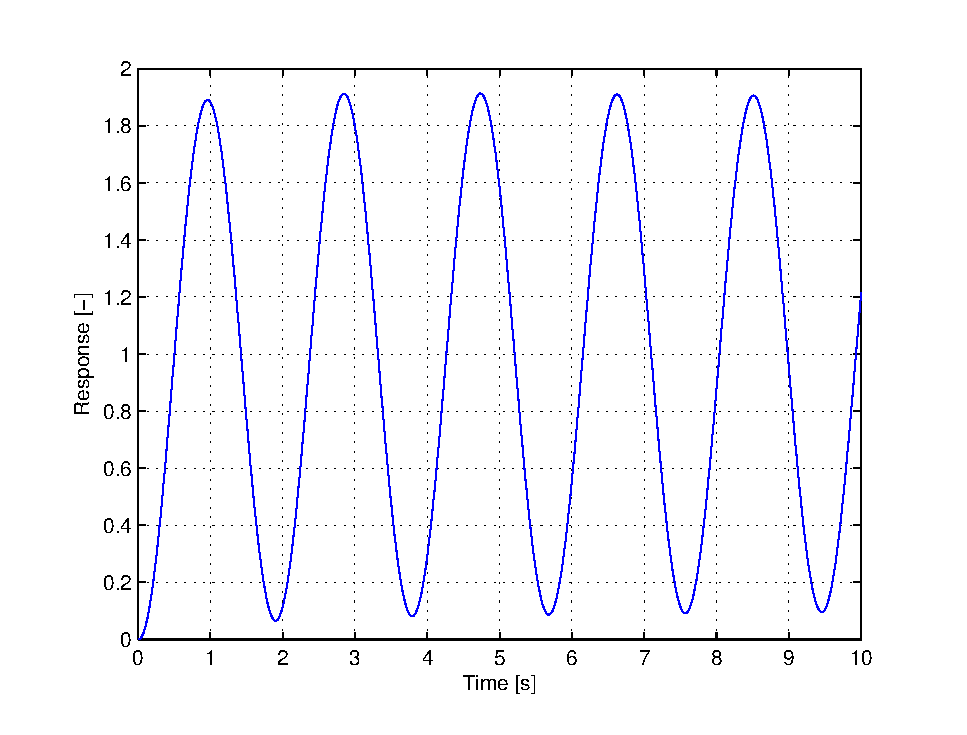
\includegraphics[width=12cm]{../res/img/2-2-0,5_resp.eps} 
	\end{center}
	\caption{Odpowiedź skokowa układu zamkniętego dla $T_{i}=T_{ig}$}
\end{figure}

\begin{figure}[!htb]
	\begin{center}
		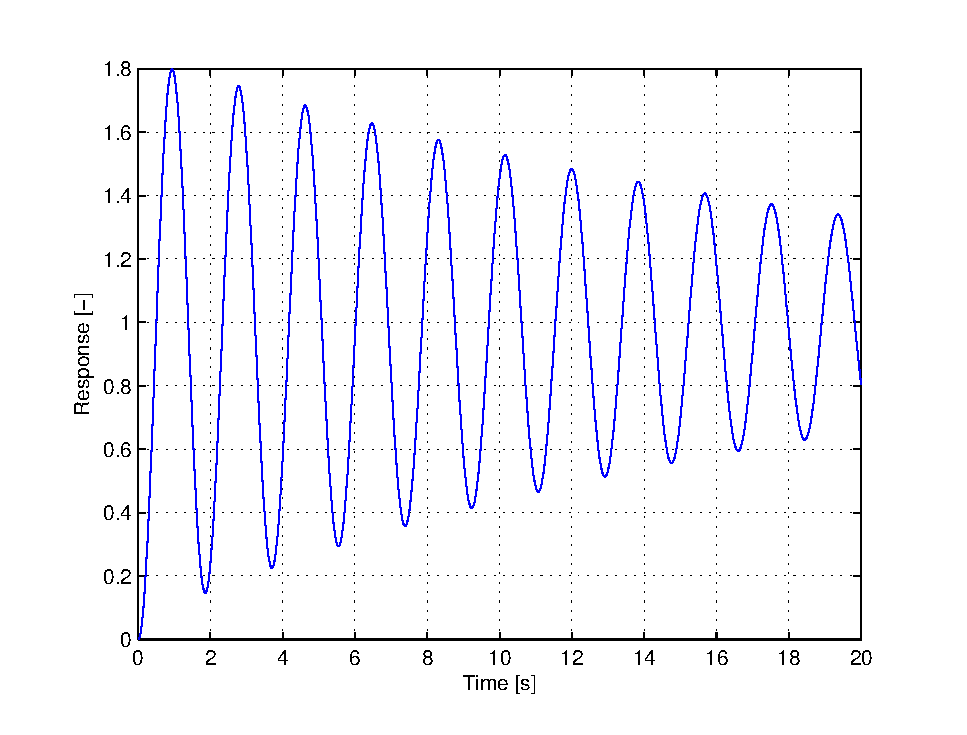
\includegraphics[width=12cm]{../res/img/2-10-0,5_resp.eps} 
	\end{center}
	\caption{Odpowiedź skokowa układu zamkniętego dla $T_{i}=T_{is}$}
\end{figure}









\newpage

\subsection{Parametr $T_d$}

Jak dla czasu zdwojenia zwiększając parametr $T_d$ regulatora
można doprowadzić do ustabilizowania układu. Metodą prób znaleźliśmy parametr
$T_d$, dla którego układ znajduje się na granicy stabilności $T_{dg}=0.55[s]$,
oraz idąc dalej - jest stabilny $T_{ds}=3[s]$. Poniżej zamieszczamy analizę
kryteriów stabilnościowych dla tak dobranych parametrów $T_d$.

\subsubsection{Kryterium Hurwitza}

Pominiemy postać transmitancji operatorowej, oraz zapis macierzy Hurwitza dla
zmienionych parametrów.

Wartości minorów dla $T_{d}=T_{dg}$ to: $\{1.02;1.92;3.62;3.13;62.66\}$,
więc kryterium stwierdza, iż układ jest stabilny. Jak w przypadku dobranego
czasu zdwojenia $T_{ig}$, pomimo iż kryterium Hurwitza mówi iż układ będzie
stabilny, będzie on się znajdować bardzo blisko granicy stabilności. Pozwala to
stwierdzić, że kryterium Nyquista jest bardziej elastyczne, ponieważ nie tylko
stwierdza czy układ jest stabilny czy nie, ale również daje pogląd na to jak
daleko od granicy stabilności się on znajduje.

Wartości minorów dla $T_{d}=T_{ds}$ to: $\{1.02;1.43;67.62;1379;27596\}$,
więc kryterium stwierdza, iż układ jest stabilny asymptotycznie.

\subsubsection{Kryterium Nyquista}

Jak widać dla $T_{d}=T_{dg}$ poniższa charakterystyka, przechodzi przez punkt
$(-1, j0)$ więc układ będzie znajdować się na granicy stabilności.

\begin{figure}[!htb] 
	\begin{center}
		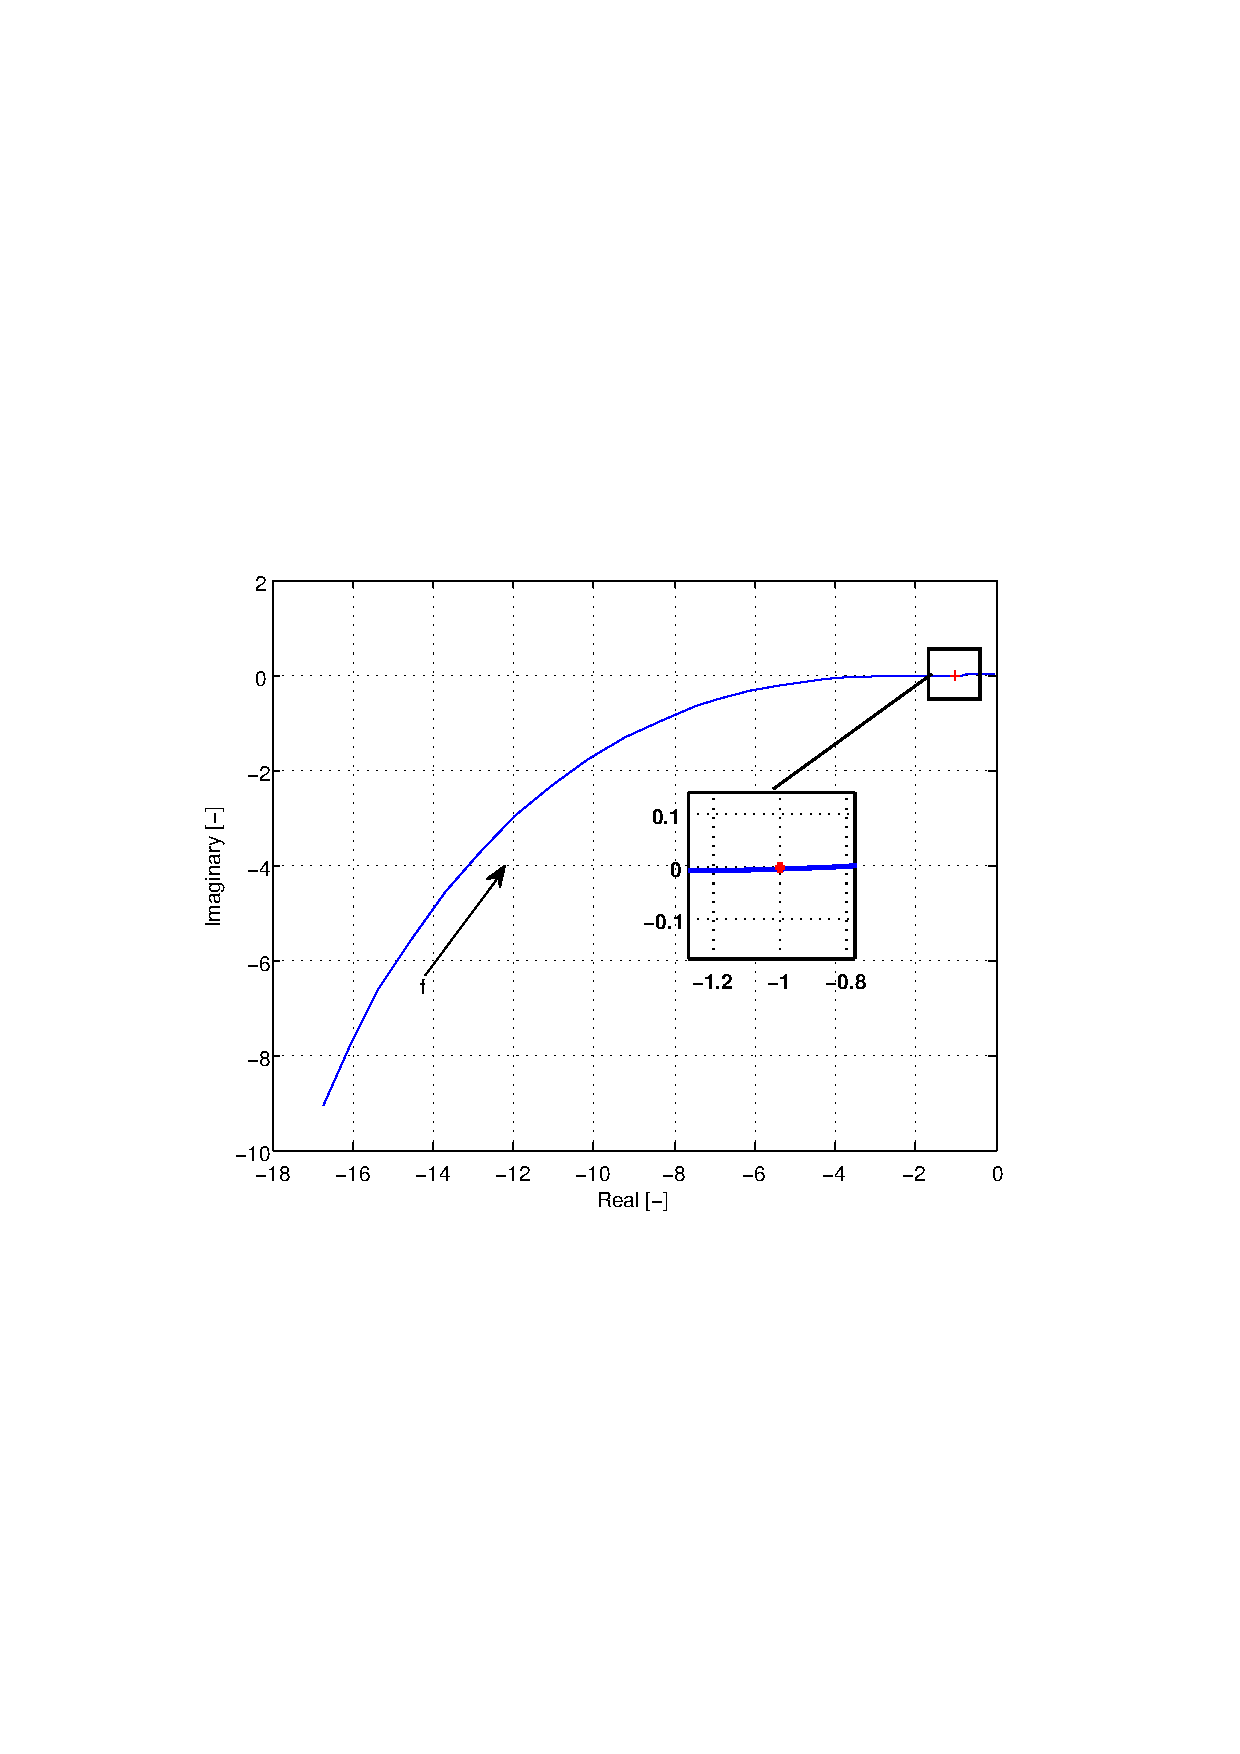
\includegraphics[trim=5cm 9cm 5cm 9cm]{../res/img/2-1-0,55_nyq.pdf} 
	\end{center}
	\caption{Charakterystyka Nyquista układu otwartego dla $T_{d}=T_{dg}$}
\end{figure}

\newpage

W przypadku $T_{d}=T_{ds}$ mijamy punkt $(-1, j0)$ mając go po lewej stronie, więc
kryterium stanowi, iż zamknięty układ regulacji będzie układem stabilnym.

\begin{figure}[!htb]
	\begin{center}
		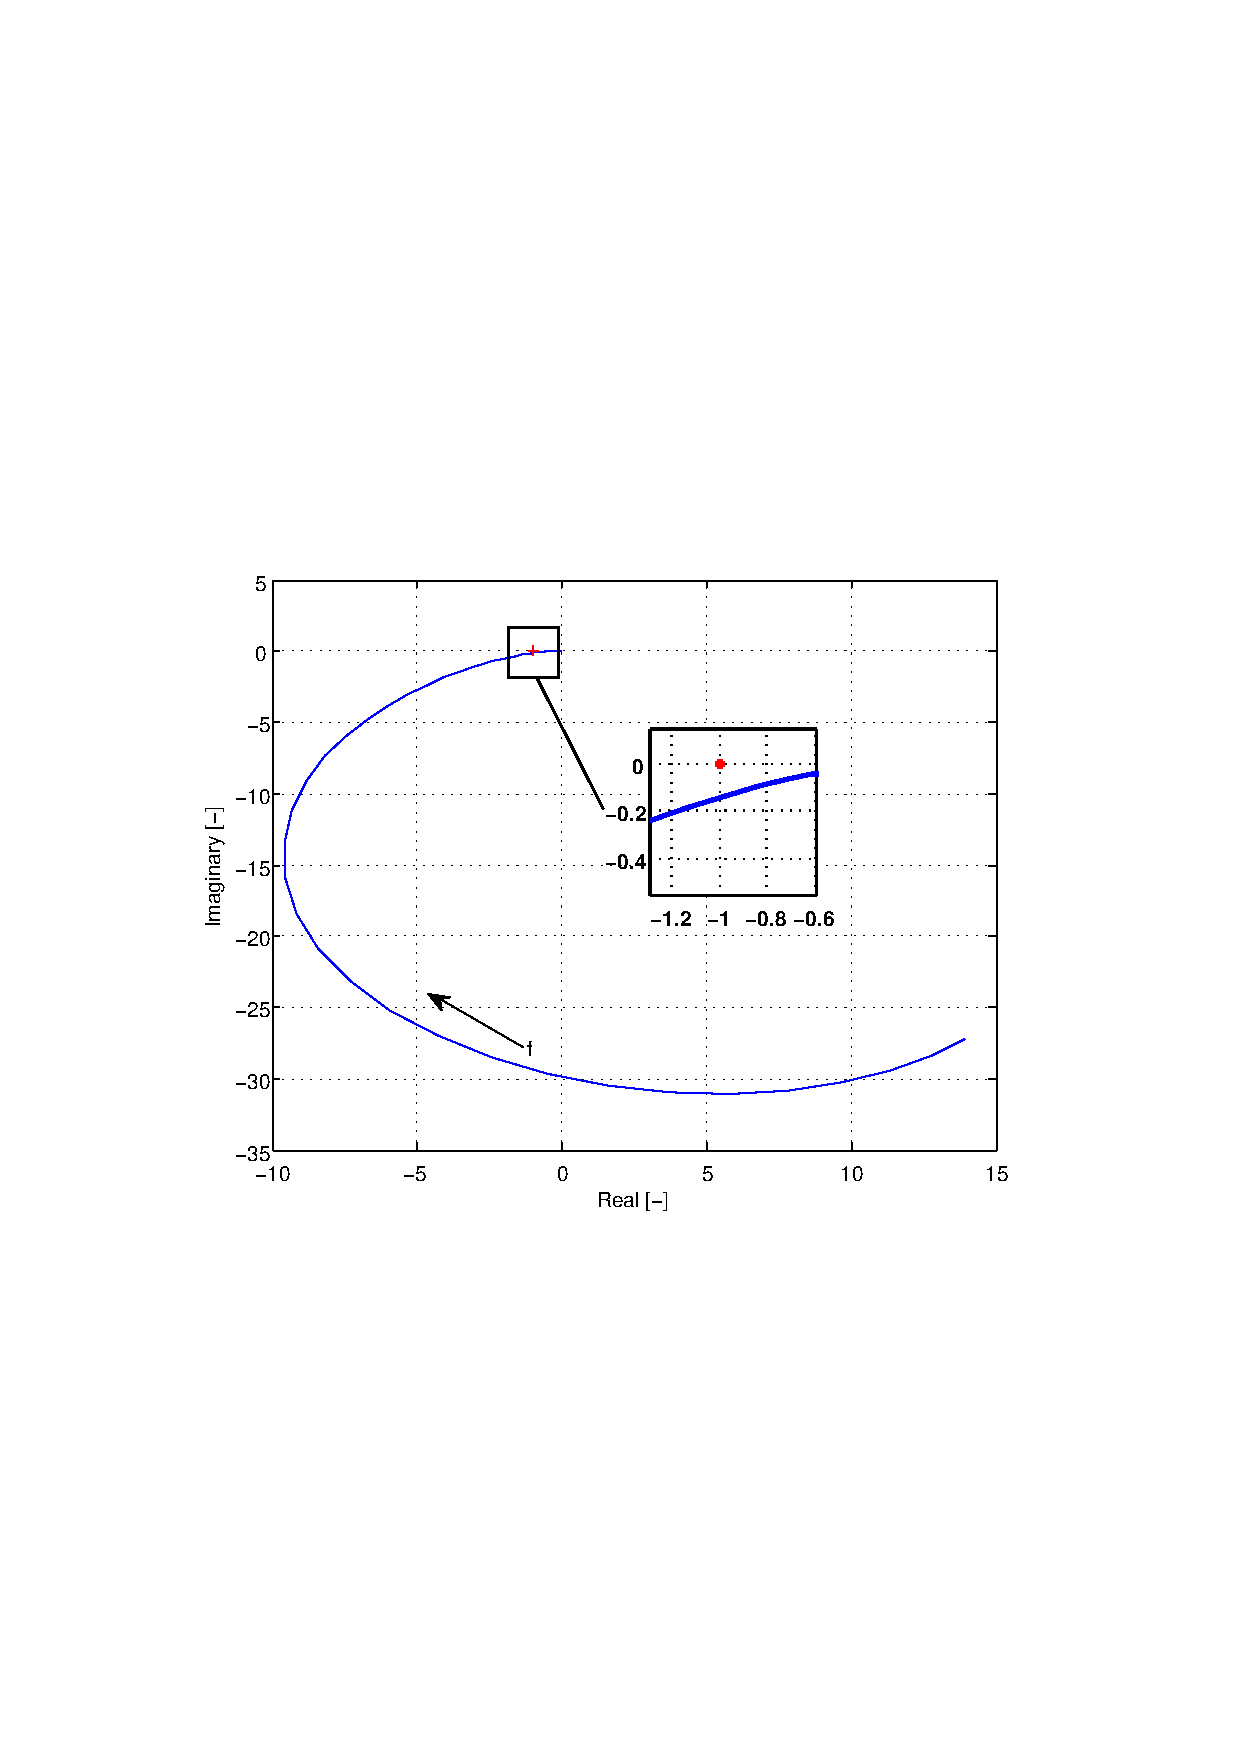
\includegraphics[trim=5cm 9cm 5cm 9cm]{../res/img/2-1-3_nyq.pdf} 
	\end{center}
	\caption{Charakterystyka Nyquista układu otwartego dla $T_{d}=T_{ds}$}
\end{figure}

\newpage

\subsubsection{Odpowiedzi skokowe}

Poniżej zamieszczone są odpowiedzi skokowe dla nastaw $T_d$ regulatora dla
których kryteria stabilności stanowią, iż układ będzie na granicy stabilności, oraz
będzie stabilny.

\begin{figure}[!htb]
	\begin{center}
		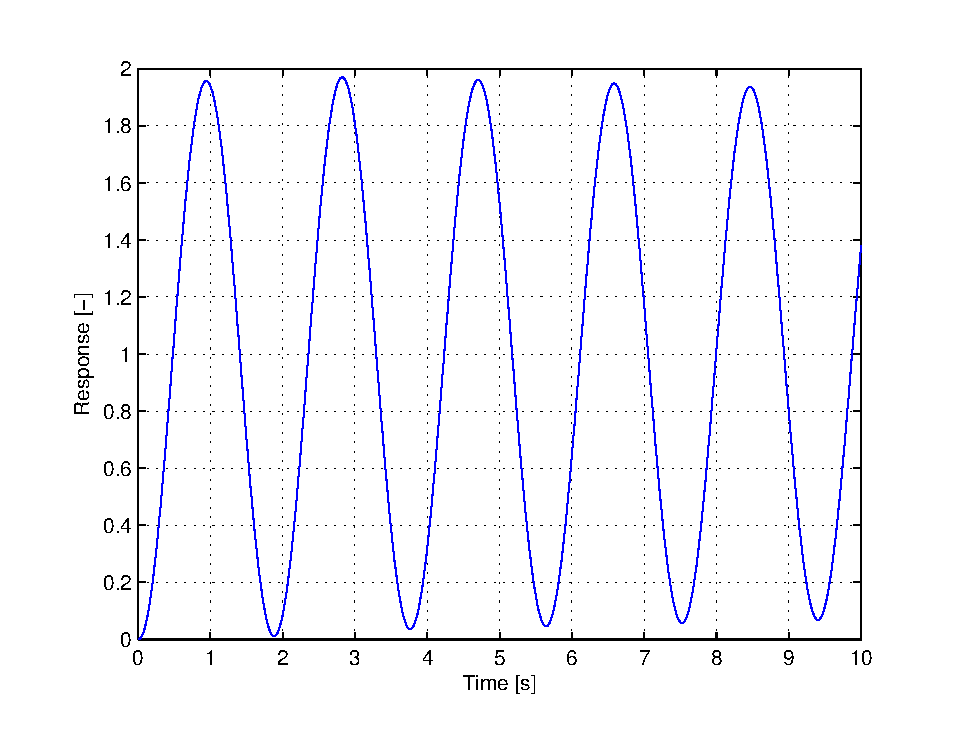
\includegraphics[width=12cm]{../res/img/2-1-0,55_resp.eps} 
	\end{center}
	\caption{Odpowiedź skokowa układu zamkniętego dla $T_{d}=T_{dg}$}
\end{figure}

\begin{figure}[!htb]
	\begin{center}
		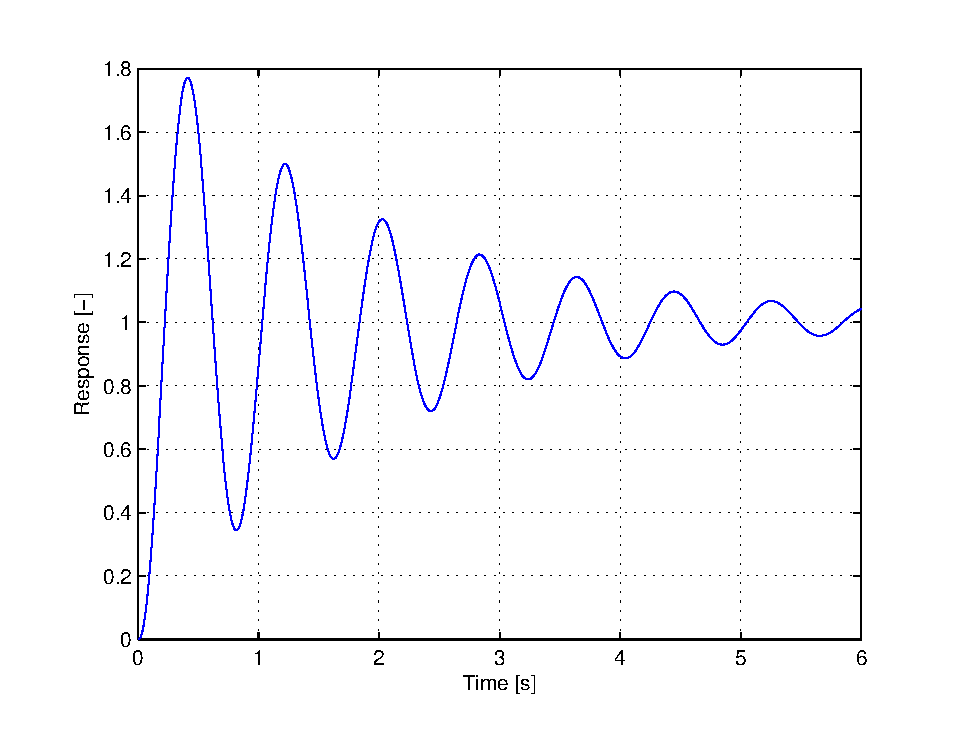
\includegraphics[width=12cm]{../res/img/2-1-3_resp.eps} 
	\end{center}
	\caption{Odpowiedź skokowa układu zamkniętego dla $T_{d}=T_{ds}$}
\end{figure}







\section{Eksperyment Zieglera–Nicholsa}

Dodatkowo postanowiliśmy sprawdzić, jakie rezultaty daje dobór nastaw regulatora
PID metodą wzmocnienia krytycznego Zieglera–Nicholsa. W tym celu ustawiamy
następujące parametry regulatora: $T_i=\infty$, $T_d=0$, oraz tak zmieniamy $k$
aby zamknięty układ regulacji znalazł się na granicy stabilności.

\begin{figure}[!htb]
	\begin{center}
		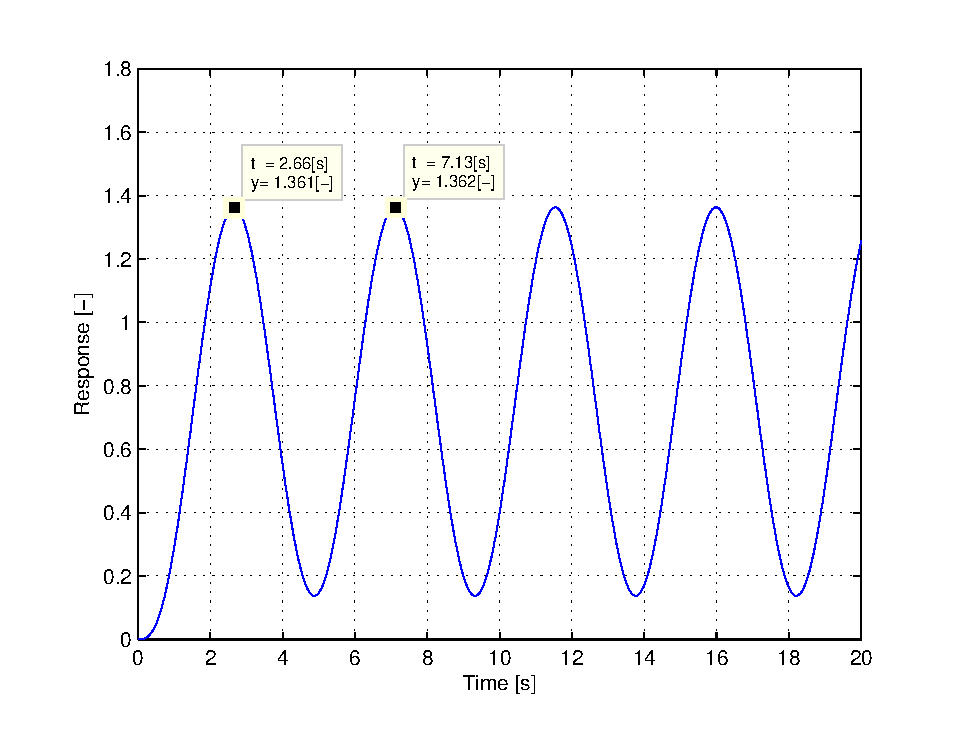
\includegraphics[width=15cm]{../res/img/0,3-inf-0_resp_kryt.eps} 
	\end{center}
	\caption{Odpowiedź skokowa układu zamkniętego dla wzmocnienia krytycznego
	$k_{kr}=0.3[-]$}
\end{figure}

Odczytujemy z odpowiedzi okres drgań sygnału wyjściowego obiektu $T=4.47[s]$.
Teraz korzystając z tabel ustawiamy parametry regulatora na
$k=0.6\cdot k_{kr}=0.18[-]$, $T_i=\frac{T}{2}=2.24[s]$,
$T_d=\frac{T}{8}=0.56[s]$

\newpage

\begin{figure}[!htb]
	\begin{center}
		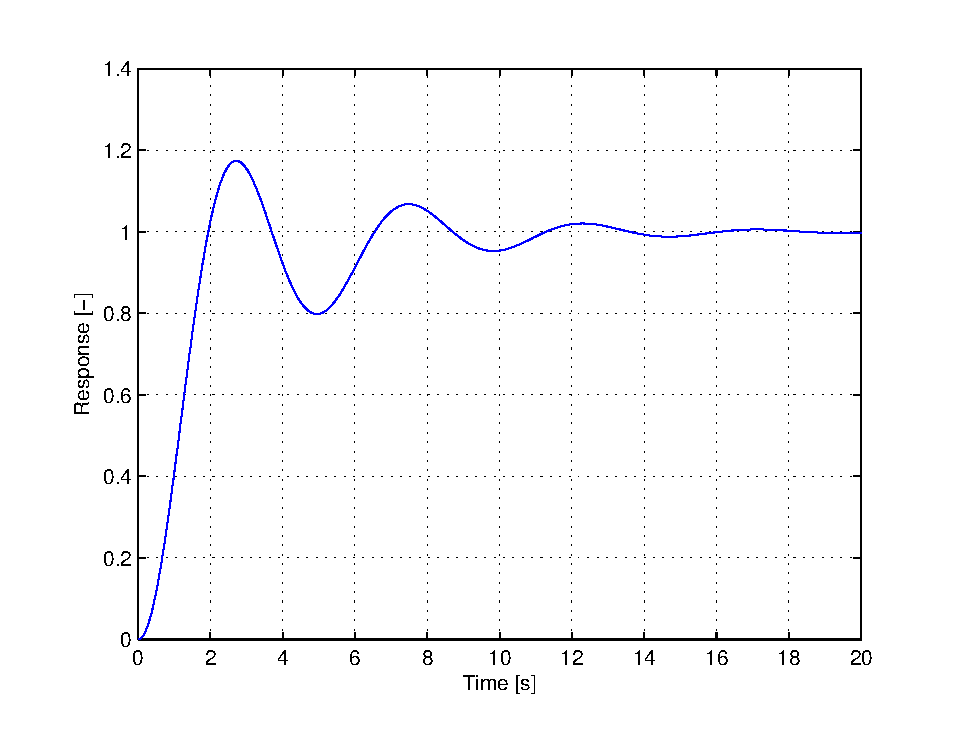
\includegraphics[width=15cm]{../res/img/0,18-2,24-0,56_resp_ZN-STD.eps} 
	\end{center}
	\caption{Odpowiedź skokowa układu zamkniętego dla nastaw dobranych metodą Z-N}
\end{figure}

Jak widać dobór nastaw metodą Z-N dała spodziewany efekt, układ zamkniętej
regulacji z tak dobranymi nastawami jest stabilny.

\section{Wnioski i spostrzeżenia}

Badane kryteria stabilności w istocie pozwalają stwierdzić, czy badany układ
jest stabilny. Obie metody, Hurwitza jak i Nyquista mają swoje wady i zalety.

Kryterium Hurwitza jest kryterium algebraicznym, więc w celu jego wykorzystania
potrzebny jest dokładny matematyczny opis badanego układu. Dodatkowo kryterium
tym ciężko stwierdzić, kiedy układ będzie się znajdować na granicy stabilności.

Kryterium Nyquista jest kryterium częstotliwościowym. O stabilności układu
zamkniętego stanowi charakterystyka częstotliwościowa układu z otwartą pętlą
sprzężenia zwrotnego. Jeśli układ otwarty jest stabilny to kryterium to jest
bardzo wygodnym do stosowania. Na podstawie charakterystyki Nyquista lub Bodego
poza samym faktem stabilności układu zamkniętego otrzymujemy informację o tym
jak blisko granicy stabilności się on znajduje.


\end{document}